\section{Empirical Study}\label{sec:experimentalResults}
We compared the unweighted (\mbox{TD-ORCS}) and weighted
(\mbox{WTD-ORCS}) versions of our top-down algorithm to LASSO and group fused \mbox{LARS} \footnote{http://cbio.ensmp.fr/~jvert/svn/GFLseg/html/} of \cite{bleakley2011group},
which are based on reformulating \eqref{eq:segmentationObjective_mu} as group
LASSO regression, and solving the optimization problem either exactly or approximately.
Both the \mbox{TD-ORCS} and \mbox{LARS} algorithms
have complexity of $\mathcal{O}\paren{nK}$.
We also report results for a Bayesian change-point detection algorithm \mbox{(BCP)}, as formulated by \cite{erdman2008fast}. We note that we experimented with a left-to-right Hidden Markov Model (HMM) for segmentation. We do not report results for this model, as its performance was inferior to the other baselines.

%--- synth-date subsection
%\input{tex_source/06_experimentalResults_synth}

\subsection{Biphones subsequences segmentation}\label{sec:biphonesSegExperiment}
In this experiment we used the \mbox{TIMIT} corpus %of
%continuous spoken English, see
\cite{garofolo1988timit}. Data include $4,620$ utterances with annotated phoneme boundaries, amounting to
more than $170,000$ boundaries. Audio was divided into frames
of $16$ms duration and
$1$ ms hop-length, each represented with $13$
\mbox{MFCC} coefficients. The task is to find the boundary between two
consecutive phonemes (biphones), and performance is evaluated as the mean
absolute distance between the detected and
ground-truth boundaries.
Since the number of segments is $K=2$ the \mbox{ORCS} and the
\mbox{TD-ORCS} algorithms are essentially identical, and the same holds for \mbox{LASSO} and \mbox{LARS}.
%We therefore report results only for \mbox{TD-ORCS}, \mbox{LARS}, and their weighted versions.
Outliers were incorporated by adding short ($0.25$ frame-length) synthetic transients to the audio source.
%composed of a few cycles of a sinusoid, modulated by an exponentially decaying amplitude envelope. Transient were added to the audio source,
The percentage
of outliers reflects the percentage of contaminated frames. Results are shown in \figref{fig:biphonesSeg_robust} as the mean error as a function of outlier percentage.
For low fraction of outliers, all algorithms perform the same, except
\mbox{WTD-ORCS}, which is slightly worse. For about $15\%$ outliers, the
performance of \mbox{W-LARS} degrades to \textapprox$27$ms mean error vs
\textapprox$22$ms for the rest. For $30\%$ outliers
both \mbox{TD-ORCS} algorithms outperform all other algorithms.
The counter-intuitive drop of error at high outliers rate for the \mbox{TD-ORCS} algorithms
might be the result of over-estimating the number of outliers. We plan to further investigate this phenomenon in future work.

We also compared our algorithm to RD, which \cite{phonemeSeg:2008} found to be the best
among five different objective functions, and was not designed for
treating outliers. In this setting (no outliers) the RD algorithm achieved
$15.1$ms mean error, while TD-ORCS achieved $13.4$ms, with $95$\% confidence interval (not
reported for the RD algorithm) of $0.1$.
%and W-LARS achieved $12.5$ms.
%For the latter algorithms the $95$\% confidence interval (not
%reported for the RD algorithm) was $0.1$.
%The outlier robust algorithm
%did not perform better than the TD algorithm in this experiment, as
%expected for the \mbox{TIMIT} corpus which is of relatively high quality.

%\begin{figure}[!t]
%        \newcommand{\factor}{.4}
%        \centering
%        
\includegraphics[width=\factor\linewidth]{figures/biphonesSeg_robust}
%      \caption{Mean error (absolute time difference to ground-truth boundary)
%      of four algorithms on TIMIT phonetic data contaminated with outliers. See text for a list of algorithms compared.}
%      \label{fig:biphonesSeg_robust}
%\end{figure}

\subsection{Radio show segmentation}
In this experiment we used a $35$ minutes, hand-annotated audio
recording of a radio talk show, composed of different
sections such as opening title, monologues, dialogs, and songs.
%In order to evaluate the segmentation results, we hand-annotated the
%different parts and this annotation was used to calculate the segmentation quality.
A detected segment boundary is considered a true positive if it falls within a tolerance window of two frames around a ground-truth boundary. Segmentation quality is commonly measured using the F measure, which is defined as $2pr/\paren{p+r}$, where $p$ is the precision and $r$ is the recall.
Instead, we used the R measure introduced by \cite{Rasanen2009}, which is more robust
to over-segmentation. It is defined as $R\triangleq1-0.5\paren{\abs{s_1}+\abs{s_2}}$, where $s_1\triangleq\sqrt{\paren{1-r}^2+\paren{r/p-1}^2}$ and $s_2\triangleq\paren{r-r/p}/\sqrt{2}$.
The R measure satisfies $R\leq1$,
and $R=1$ only if $p=r=1$.
%Unlike the F measure, the R measure takes into account over-segmentation. In what follows we report the $R$ measure, as the %$F$ measure did not convey qualitatively different information.

\paragraph{Signal representation} A common representation in speech analysis is the MFCC coefficients mentioned in \secref{sec:biphonesSegExperiment}. However, this representation is computed over time windows of tens of milliseconds, and therefore it is not designed to capture the characteristics of a segment with length in the order of seconds or minutes. We therefore apply post-processing on the MFCC representation. First, the raw audio is divided
into $N$ non-overlapping blocks of $5$ seconds duration, and the MFCC coefficients are computed for all blocks $\braces{S_j}_{j=1}^N$. We used 13 MFCC coefficient with $25$ms window length and $10$ms hop length. Then a Gaussian Mixture Model (GMM) $T_j$ with $10$ components and a diagonal covariance matrix is
fitted to the $j$th block $S_j$. These parameters of the GMM were selected using the Bayesian Information Criterion (BIC). The log-likelihood matrix $A$
is then defined by $A_{ij}=\log\prob{S_j|T_i}$. %Experimentally we notice
%that the symmetrized log-likelihood matrix $A+A^T$ results in worse
%segmentation measure, so we use the non-symmetrized matrix $A$.
The clean feature matrix (no outliers) is shown in
\figref{fig:likemat}, where different segments can be discerned.
%corresponding to different speakers, a song, etc.
%\begin{figure}[!t]
%        \newcommand{\factor}{.3}
%        \centering
%        \subfigure[Likelihood matrix\label{fig:likemat}]{
\includegraphics[width=\factor\linewidth]{figures/GMM_likeMat}}
%        %\subfigure[Maximal R measure vs. \% of outliers\label{fig:maxRscoreSynthOL}] {\includegraphics[width=\factor\linewidth]{figures/outliersRobust_synth_RvsP}}
%        \subfigure[Maximal R measure vs. \% of outliers\label{fig:maxRscoreAudiohOL}]{\includegraphics[width=\factor\linewidth]{figures/outliersRobust_audio_RvsP}}
%       \caption{ (a) $A_{ij} = \log\prob{S_j|T_i}$ is the
%         log-probability of segment $j$ given the GMM model fitted to segment $i$.
%         \subref{fig:maxRscoreAudiohOL} Maximal R measure vs. percentage of
%         outliers, for the outlier-robust (ORCS), unweighted and weighted outlier-robust top-down (TD-ORCS, W-TD-ORCS), weighted LARS (W-LARS), and bottom-up (BU) algorithms. Outliers were added to the raw audio.}
%\end{figure}
Since using the columns of $A$ as features yields a dimension growing %linearly
with $N$, we randomly choose a subset of $d=100$ rows
of $A$, and the columns of the resulting matrix $X\in\mathbb{R}^{d\times N}$ are the
input to the segmentation algorithm.
We repeat the experiment for different number of outliers, ranging between $0\%$ and $16\%$ with intervals of $2\%$.
%Details regarding the outliers generation are given below.
Outliers were added to the raw audio. A given percentage of outliers refers to the relative
number of blocks randomly selected as outliers, to which we add a $5$ seconds recording of repeated hammer strokes,
normalized to a level of $0$dB SNR.

\paragraph{Algorithms} We consider the Outlier-Robust
Convex Sequential (ORCS) segmentation, and its top-down versions (weighted and unweighted)
which we denote by WTD-ORCS and TD-ORCS, respectively.
We compare the performance to three other algorithms. The first is a greedy bottom-up (BU)
segmentation algorithm, which minimizes the sum of squared errors on
each iteration. The bottom-up approach has been successfully used in
tasks of speech segmentation \cite{qiao:2012study,gracia:2011hierarchical}.
The second algorithm is the W-LARS algorithm of \cite{bleakley2011group}. The third algorithm is a Bayesian change-point detection algorithm (BCP), as formulated by \cite{erdman2008fast}.
%, which we compared to in \secref{sec:synthDataExperiment} as well.
A solution path was found as follows.
%For the CS algorithm, $250$ values of
%$0<\lambda<\lambda^*$ were sampled on a logarithmic scale.
For the ORCS algorithm, a $35\times35$ parameter grid was used, where
$0<\gamma<\gamma^*$ was sampled uniformly, and for each $\gamma$ value,
$0<\lambda<\lambda^*\paren{\gamma}$ was sampled logarithmically, where
$\lambda^*\paren{\gamma}$ is the critical value for $\lambda$ for a
given choice of $\gamma$ (see \secref{sec:robust_top_down} for details). For the TD-ORCS, W-LARS, and BU algorithms,
$K=2\comdots 150$ number of segments were used as an input to the
algorithms. For the TD-ORCS algorithm, where the number of required
outliers is an additional input parameter, the correct number of
outliers was used. For the BCP algorithm, a range of thresholds on the posterior probability of change-points was used to detect a range of number of segments. As is evident from the empirical results below, the ORCS algorithm can
achieve high detection rate of the outliers even without knowing their
exact number a-priori. Furthermore, we suggest below a way of
estimating the number of outliers.
%Experimenting with a range of the number of outliers as input
%is left to a future work.
For each algorithm, the maximal R measure over all parameters range
was used to compare all algorithms.

\paragraph{Results}
Results are shown in
\figref{fig:maxRscoreAudiohOL} as the maximal R measure achieved versus the percentage
of outliers, for each of the algorithms considered. It is evident that the
performance of the BU and BCP algorithms decreases significantly as
more outliers are added, while the outlier-robust ORCS algorithm
keeps an approximately steady performance. Our unweighted and weighted TD-ORCS algorithms
achieve the best performance for all levels of
outliers. Results for LARS algorithm are omitted as it did not perform better than other algorithms.
We verified the ability of our algorithms to correctly detect outliers
by calculating the R measure of the outliers detection of the ORCS algorithm, with zero
length tolerance window, i.e a detection is considered a true-positive
only if it exactly pinpoints an outlier.
The R measure of the detection was evaluated on the $\gamma$, $\lambda$ parameter
grid, as well as the corresponding numbers of detected outliers. Results for the representative case of $p=10\%$ outliers are shown in
\figref{fig:detRateAudio}.
It is evident that a high R measure ($>0.9$) is attained on a range of
parameters that yield around the true number of outliers. We conclude that one does not
need to know the exact number of outliers %in a given data sample
in order to use the ORCS algorithm, and a rough estimate is enough. Some
preliminary results suggest that such an estimate can be approximated
from the histogram of number of detected outliers
%, or the frontier in the number of outliers plots
(i.e. \figref{fig:nOutliersAudio}).
%Finally, initial results showed that
%if the algorithm tries to detect more outliers than exist, the
%performance may slightly improve.

\begin{figure}[!t]
        \newcommand{\factor}{.45}
        \begin{minipage}{.47\textwidth}
            \centering
            \subfigure[Likelihood matrix\label{fig:likemat}]{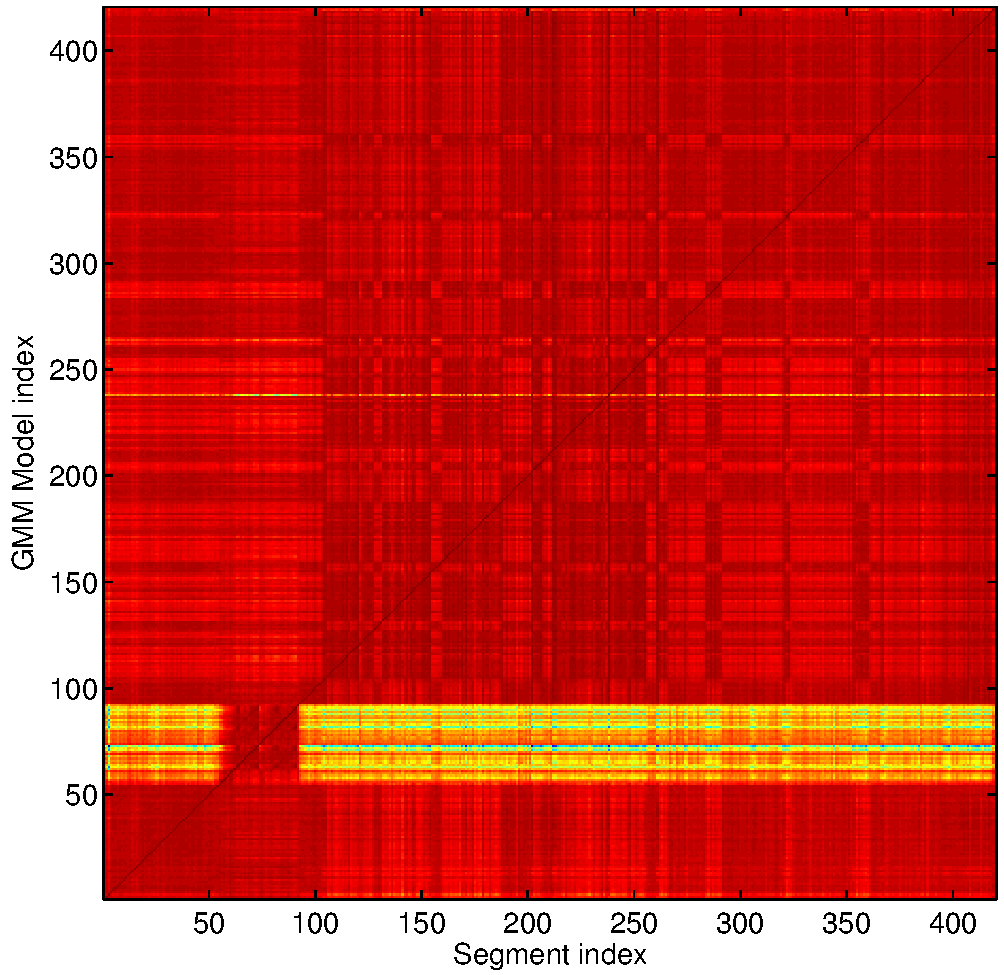
\includegraphics[width=.44\linewidth]{figures/orig_in_color/GMM_likeMat}}
            \subfigure[Maximal R vs. \% of outliers\label{fig:maxRscoreAudiohOL}]
            {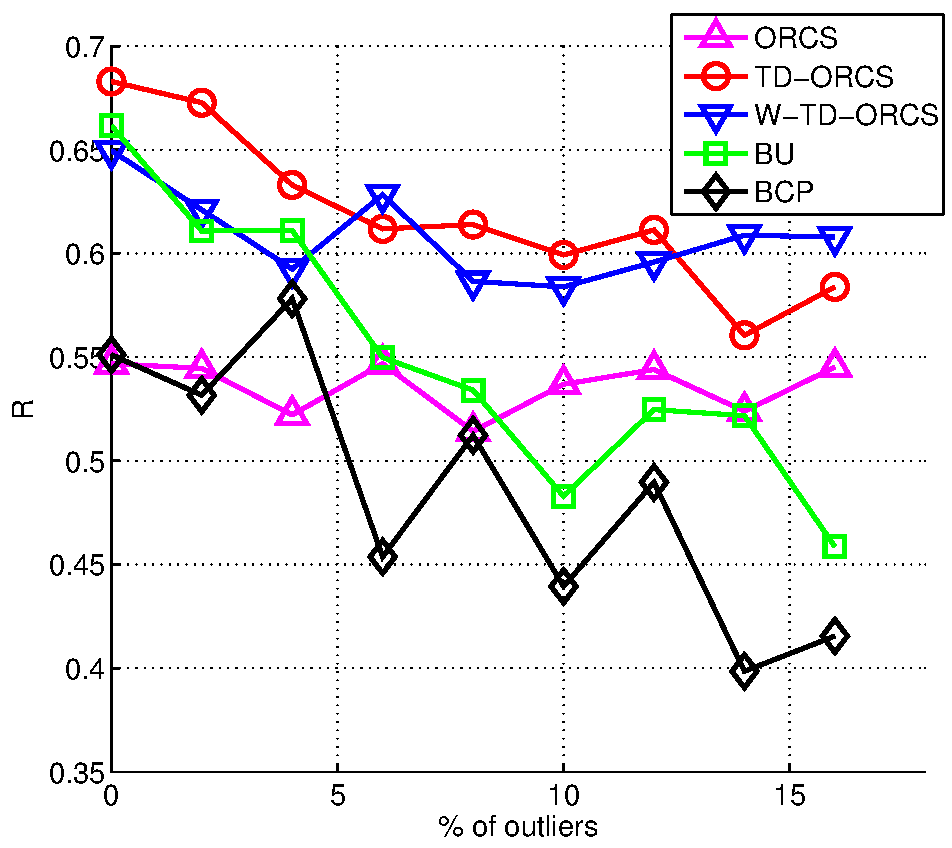
\includegraphics[width=\factor\linewidth]{figures/orig_in_color/outliersRobust_audio_RvsP_incBCP}}
            \caption{(a) $A_{ij}$ % = \log\prob{S_j|T_i}$
            is the log-probability of segment $j$ given the
            GMM fitted to segment $i$.
            %\subref{fig:maxRscoreAudiohOL}
            (b) Maximal R measure vs. percentage of
            outliers. See text for algorithms details.
            %, for the outlier-robust (ORCS), unweighted and weighted outlier-robust top-down (TD-ORCS, W-TD-ORCS), weighted LARS (W-LARS), and bottom-up (BU) algorithms. Outliers were added to the raw audio.
            }
            \centering
            \subfigure[R measure\label{fig:detRateAudio}]{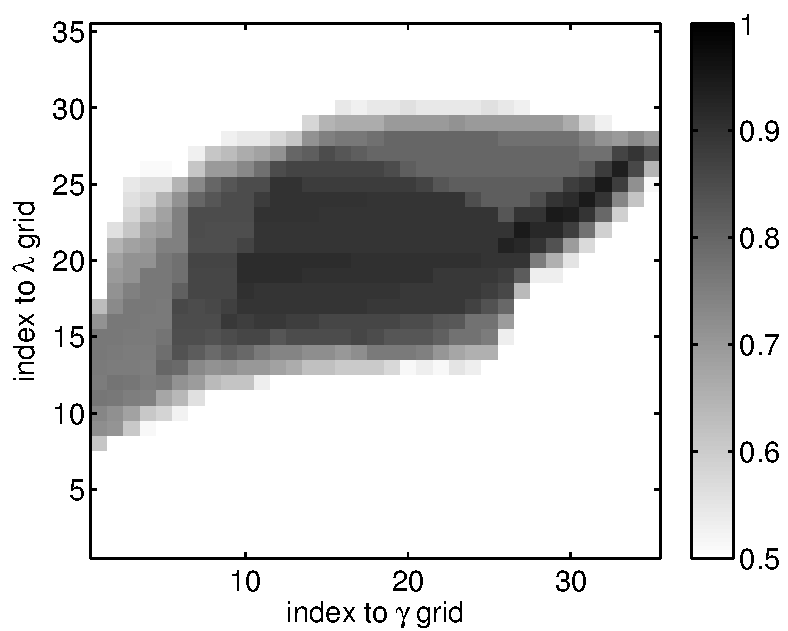
\includegraphics[width=\factor\linewidth]{figures/orig_in_color/audioOlDetectionRate_10p}}
            \subfigure[Number of detected outliers\label{fig:nOutliersAudio}]{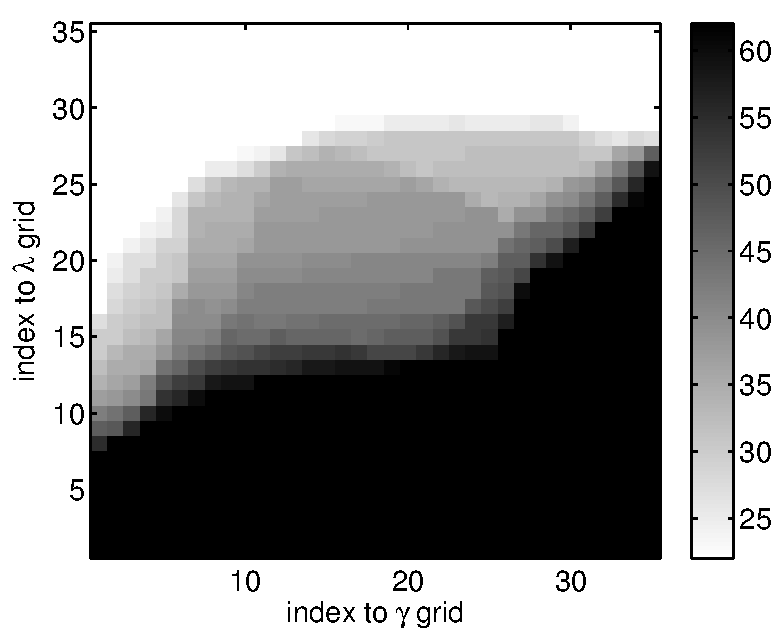
\includegraphics[width=\factor\linewidth]{figures/orig_in_color/audioOlNumOutliers_10p}}
            \caption{%\subref{fig:detRateAudio}
            (a) Outliers detection quality by the ORCS algorithm, quantified using the R measure of outliers detection. R is evaluated on a $35\times35$ parameter grid, for $10\%$ outliers.
            %\subref{fig:nOutliersAudio}
            (b) The corresponding number of detected outliers.}
            \label{fig:detectionRate}
        \end{minipage}
\end{figure}

% \begin{figure*}[!t]
%         \newcommand{\factor}{.24}
%         \centering
%         \begin{subfigure}{\factor\linewidth}
%                 \includegraphics[width=\linewidth]{figures/synthOlDetectionRate_10p}
%                 \caption{R measure}\label{fig:detRateSynth}
%         \end{subfigure}
%         \begin{subfigure}{\factor\linewidth}
%                 \includegraphics[width=\linewidth]{figures/synthOlNumOutliers_10p}
%                 \caption{Number of detected outliers}\label{fig:nOutliersSynth}
%         \end{subfigure}
%         \begin{subfigure}{\factor\linewidth}
%                 
\includegraphics[width=\linewidth]{figures/audioOlDetectionRate_10p}
%                 \caption{R measure}\label{fig:detRateAudio}
%         \end{subfigure}
%         \begin{subfigure}{\factor\linewidth}
%                 
\includegraphics[width=\linewidth]{figures/audioOlNumOutliers_10p}
%                 \caption{Number of detected outliers}\label{fig:nOutliersAudio}
%         \end{subfigure}
%        \caption{Outliers detection quality by the ORCS algorithm, quantified using the R measure of outliers detection. R is evaluated on a $35\times35$ parameters grid, for $10\%$ (42 data samples) synthetic outliers (\subref{fig:detRateSynth}) and audio-level outliers (\subref{fig:detRateAudio}). Also shown are the corresponding number of detected outliers (\subref{fig:nOutliersSynth}, \subref{fig:nOutliersAudio})}
%        \label{fig:detectionRate}
%       \vspace{-.3cm}
% \end{figure*}
